\chapter{Linear Algebra and Neural Networks}\label{ch_linear_algebra}
\chapterauthor{Jeff Yoshimi, Scott Hotton}

% Also see "indexing hell" comment at  http://neuralnetworksanddeeplearning.com/chap2.html

% Identity matrix

% NN discovers faster matrix product: https://www.nature.com/articles/s41586-022-05172-4. Oddly meta.

In this chapter, we review some basic concepts of linear algebra with an 
emphasis on how they can be applied to the study of neural networks. This can be viewed as a transition from the formal structure of single nodes and weights, to the formal structure of \emph{lists} and \emph{tables} of nodes and weights. In particular, we  consider vectors and matrices, which allow us to describe the behavior of groups of nodes and weights in a compact way.

Linear algebra also facilitates a powerful geometric framework for \emph{visualizing} the structure and dynamics of a neural network. The properties of a set of inputs and whether they can be properly classified is an example of something that is  more intuitively understandable when the input vectors are visualized as points in a space. Chapter \extref{ch_act_functions} notes that whenever the ``play''  button 
\includegraphics[scale=.5]{./images/Play.png} is pressed in Simbrain, some dynamical process is simulated. The framework of linear algebra makes it possible to visualize the changing activations of a set of nodes, or the changing strengths of a set of weights, as a moving point in a space. This approach to thinking about neural networks uses \emph{dynamical systems theory}, discussed in chapter \extref{ch_dst}, and can be used to think about many features of neural network models in an intuitive way.\footnote{For a quick demonstration of this way of visualizing network dynamics, try running the simulation \emph{highDimensionalProjection.bsh}. The dynamics of the network is visible in the projection component.}  

\section{Vectors and Vector Spaces}\label{sect_vector}

% This needs to be done in an intuitive way first, then formalized
    Linear algebra is the study of vector spaces. Vector spaces are abstract
mathematical systems that turn out to be extremely useful for describing the 
structure and dynamics of neural networks. A \glossary{vector space} is a 
collection of objects called \glossary{vectors} along with mathematical 
operations that we can perform with the vectors.\footnote{You may have heard 
that vectors are geometric objects that have a magnitude and a direction. You 
may have seen them represented by an arrow or directed line segment. These 
different points of view on vectors supplement rather than contradict each 
other.}  For instance, we can add two vectors together to get another vector. There is also a type of 
multiplication that can be performed between a vector and a \glossary{scalar}. The term ``scalar'' is used for those numbers that are allowed to be 
multiplied with a vector. We will focus on the case where scalars are real numbers, like $2$, $-1.2$, or $5.9$. If the scalars are the set of real numbers, then the 
vector space is called a {\em real vector space}. We will only work with real
vector spaces. A more formal definition for a vector space is discussed in 
Sect. \ref{S:LinearAlgebraAppendix}. 

We will represent vectors as ordered lists of scalars.\footnote{ Many classes of mathematical objects satisfy the formal definition
of a vector space, and thus many objects can be vectors. The ordered lists we consider here are an especially convenient type of vector.} Each of the scalars in the list is called a \glossary{component} 
of the vector. A list with 2 components is called an {\em ordered pair}. A 
list with 3 components is called an {\em ordered triple}. More generally, a
list with $n$ components is called an {\em $n$-tuple}. We can refer to the
members of a vector in this sense  as its ``first component'',  ``second component'', etc.
A vector in the sense of an $n$-tuple is often 
written out as a comma-separated list of numbers surrounded by parenthesis. 
For example, here are four vectors:
\begin{equation*}
    (0,0) \quad (0,1) \quad (1,0) \quad (1,1) 
\end{equation*}

% TODO: Expand this as we use this more and decide if any convention regarding indices should be given now.
   We sometimes adopt the convention of writing vectors using bold-faced 
lower-case letters, for example $\mathbf{a}_i$ for a  vector of input values, 
$\mathbf{t}$ for a vector of target values, or $\mathbf{a}_4$ for the 
activation vector in the fourth node-layer of a feed-forward network.  By 
contrast non bold-faced, italic lower-case letters are usually reserved for 
components of vectors, and the subscript indicates which component. For 
example, $a_2$ could designate the second component of an activation vector 
$\mathbf{a}$.

When the components of a vector are written horizontally, from left to right,
it is called a {\em row vector}. The ordered pairs shown above are row 
vectors. The components can also be written out vertically, from top to 
bottom, in which case the vector is called a {\em column vector}.\footnote{The choice of whether
to use a row or a column vector to represent an abstract vector is primarily a matter of 
convenience or convention.} Commas are usually 
not written in column vectors because it is clear what the components are. For 
example, here are four column vectors:
\begin{small}
\begin{equation*}
\begin{pmatrix}
0 \\
0
\end{pmatrix} 
\quad 
\begin{pmatrix}
0 \\
1
\end{pmatrix} 
\quad 
\begin{pmatrix}
1 \\
0
\end{pmatrix} 
\quad 
\begin{pmatrix}
1 \\
1
\end{pmatrix} 
\end{equation*}
\end{small}
The number of components in a vector can be any positive integer. If there is
only one component, then the vector is essentially just a scalar.

   For any positive integer $n$, the set of all $n$-tuples forms a vector space.
The integer $n$ is called the \glossary{dimension of a vector space}. For 
example, the set of all of ordered pairs of real numbers is a 2 dimensional 
real vector space $\real^2$. The set of all ordered triples is a 3 dimensional real 
vector space $\real^3$. The set of all possible activations for a network with 172 nodes is a subset of  $\real^{172}$.

   The components of a vector can be thought of as the coordinates of a point
in Euclidean geometry. The components of a vector can be used to locate a
point by starting at the origin and moving parallel to each axis by the 
amount specified by the corresponding component. To locate the point corresponding to the vector 
$(3,4)$, for example, we move $3$ units to the right along the 
horizontal axis and $4$ units upwards along the vertical axis. In this way a 
2 dimensional real vector space can be thought of as an Euclidean plane (see 
figure \ref{2d}).\footnote{There is a legend (probably fabricated, but pedagogically useful nonetheless) 
that the philosopher Ren{\'{e}} Descartes 
 came up with his proof that given a point in the plane there are unique coordinates for that 
 point (and given a pair of coordinates there is a unique point in the plane) 
 while observing flies on his ceiling. He 
 noticed that the position of the flies on the ceiling could be described by 
 superimposing a kind of grid on the ceiling---for example: there's a fly at 
 $(3,4)$, 3 units to the right, and 4 units up; there's a fly at 
 $(-2,-1)$, 2 units to the left, and 1 unit down; and there's another at 
 $(4,-2)$, 4 units to the right, and two units down (see figure \ref{2d}).} 
 
 % This is useful in Simbrain but the connection is a bit lost here 
For 2-dimensional spaces, finding your way around is a bit like using an ``Etch a sketch'' toy\footnote{\url{https://en.wikipedia.org/wiki/Etch_A_Sketch}.}, where you move a tracing point around in a space using one knob for left-and-right ($x$-values) and one knob for up and down ($y$-values). If you plot the activation space of two nodes in Simbrain and adjust the activations of the two nodes, this analogy is useful for understanding what is happening.

\begin{figure}[h]
\centering
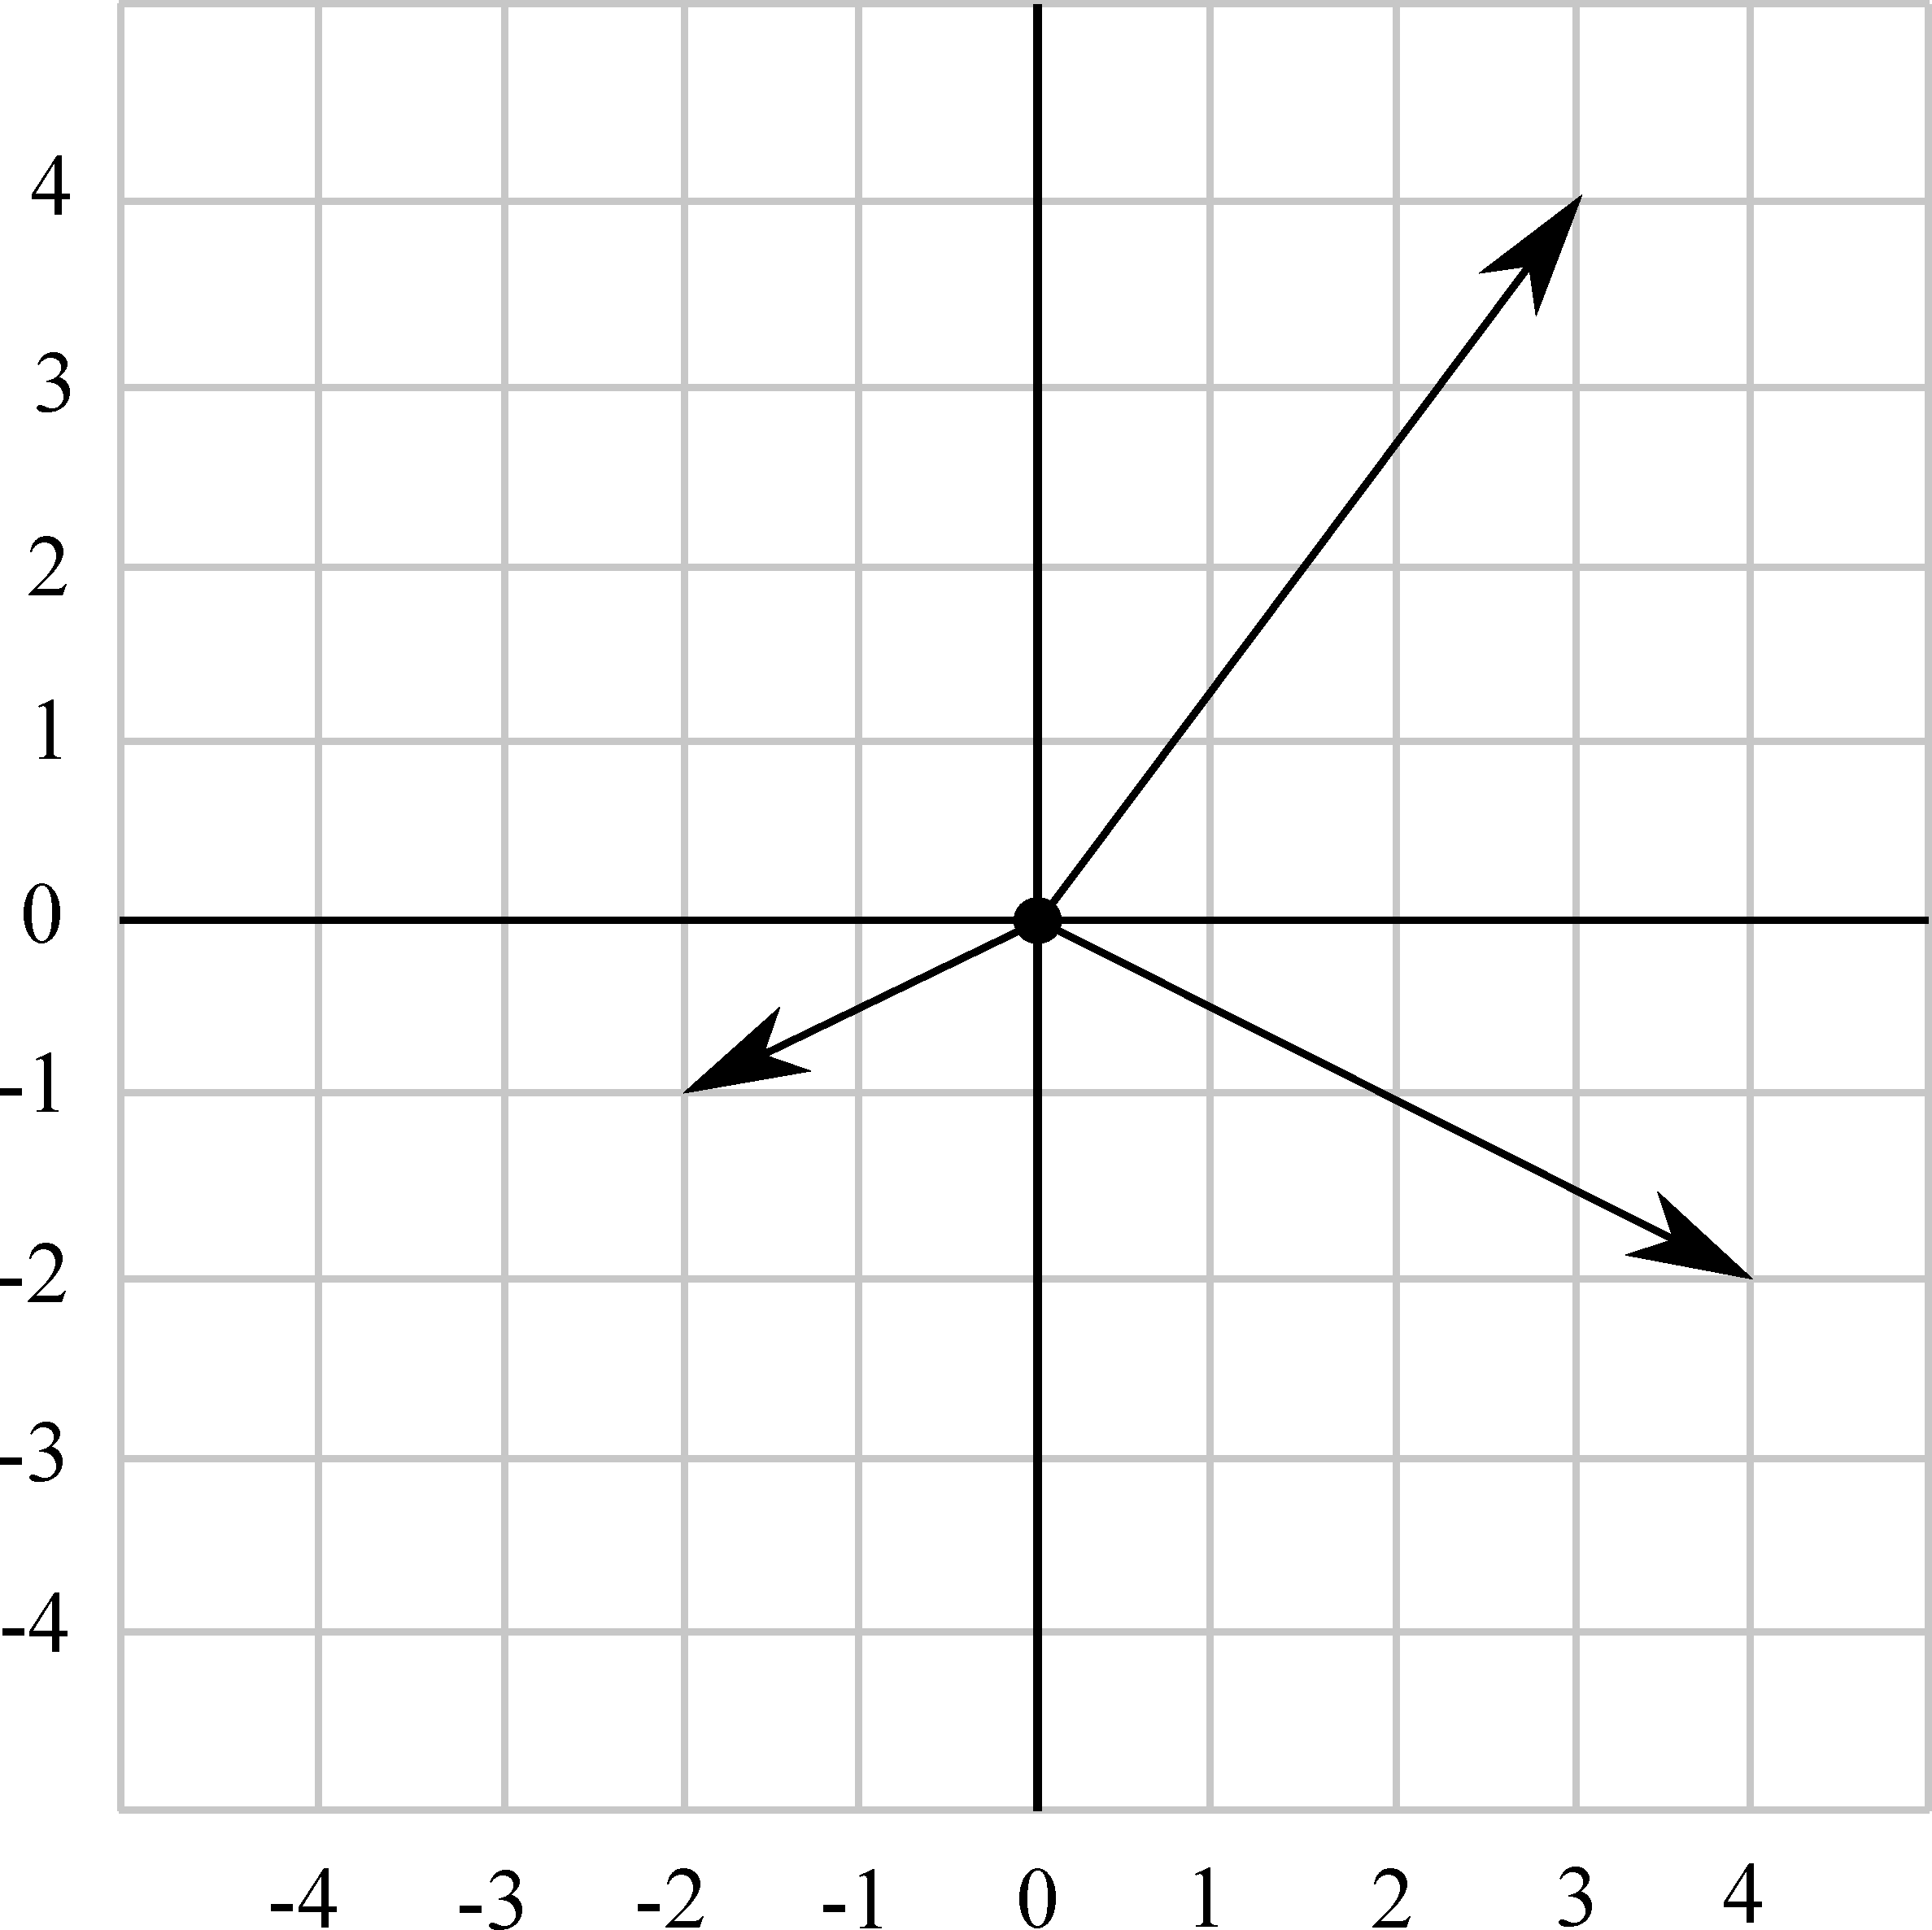
\includegraphics[scale=0.175]{./images/grid2.png}
\caption[Scott Hotton.]{Each vector in a 2 dimensional vector space is associated to a point 
in the Euclidean plane by treating the components of the vector as the 
coordinates of the point. Try to find the vectors $(3,4)$, $(-2,-1)$, and 
$(4,-2)$.} 
\label{2d}
\end{figure}

   The number of dimensions of the vector spaces that arise in the study of 
neural networks can be much larger than 3. We we can not geometrically visualize these higher-dimensional spaces directly. To work mathematically in 
these spaces, it is helpful to keep in mind that our starting point is the 
$n$-tuples, which are just lists of numbers. From this standpoint, the 4 
dimensional real vector space we work with is just the set of all $4$-tuples of
real numbers, and the 5 dimensional real vector space we work with is just the 
set of all $5$-tuples of real numbers. Here are some vectors in a 5 
dimensional vector space:
\begin{equation*}
    (0,-1, 1, 0.4, 9)  \qquad
    (-1, 2, 4, -3, 9)  \qquad 
    (0, 0, 0, -1, -1 ) \qquad
    (0, -1, 0, -1, 0 ) 
\end{equation*}
We can keep going. The vectors that make up a 100 dimensional vector space are 
just lists of 100 numbers. The vectors that make up a billion dimensional 
vector space are just lists of a billion numbers. 

   Real vector spaces with more than 3 dimensions cannot be seen directly, but 
objects in them can be \emph{projected} to lower dimensional real vector spaces 
where they can be visualized. We will discuss methods of projection from 
spaces with more than 3 dimensions in Sect. \ref{S:dimReduction}.\footnote{Here
again the Simbrain simulation \emph{highDimensionalProjection.bsh} is helpful.
When you run the simulation, a sequence of points in a 25 dimensional space 
appears. Each point corresponds to a vector. If you hover the cursor over any
one of the points, you will see the list of 25 numbers (the 25 activation levels
for the network) that correspond to that point.}

\section{Vectors and Vector Spaces in Neural Networks}\label{S:dimReduction}

   Vectors are frequently used to describe lists of activations, weights, and other quantities associated with neural networks. 

\begin{figure}[h]
\centering
\raisebox{-0.5\height}{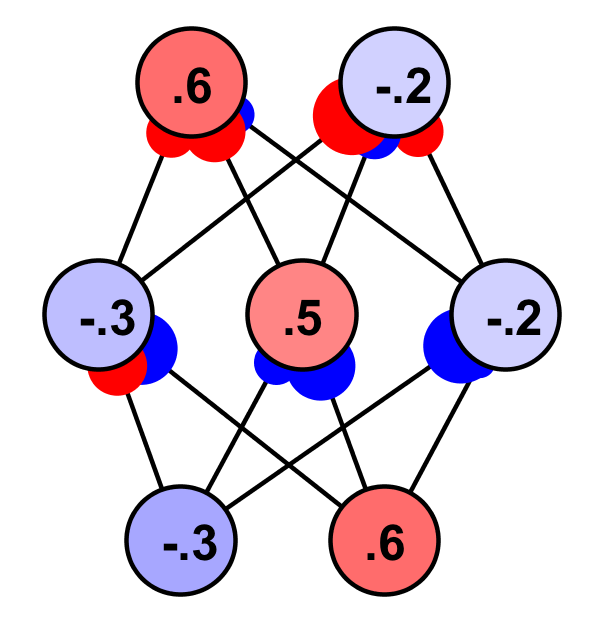
\includegraphics[scale=.5]{./images/ff.png}}
\hspace*{1in}
\raisebox{-0.5\height}{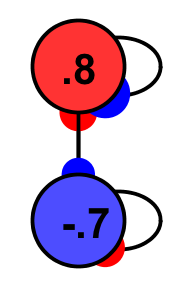
\includegraphics[scale=.3]{./images/recurrent.png}}
\caption[Simbrain screenshots.]{A feed forward and recurrent network in Simbrain. Try to identify the dimensionality of the activation space, input space, hidden unit space, output space, and weight spaces of each network. Left: A feed-forward neural network with activations showing. Right: A 2-node recurrent network with activations showing.}
\label{ffRecurrent}
\end{figure}

% TODO: Run the bold-faced notation through
  The activations of a neural network's $n$ nodes can be described by an \glossary{activation 
vector} with $n$ components, one for each activation value. For example, if we index the nodes of the feed-forward network in figure \ref{ffRecurrent} (Left) from the bottom to the top and left to right (as in figure \ref{labelledNets}), then that networks' activation vector is $(-0.3,0.6,-0.3,0.5,-0.2,0.6,0.2)$. This 
is a vector in a 7 dimensional vector space. A vector space of activation 
vectors is called an \glossary{activation space}. The feed-forward network in figure \ref{ffRecurrent} (Left)  network has a 7 dimensional activation space.

Activation spaces are especially useful in studying recurrent networks. If we index the nodes of the recurrent network in figure \ref{ffRecurrent} (Right) from top to bottom (as in figure \ref{labelledNets}), then its activation vector is $(0.8,-0.7)$. This is a vector in a 2 dimensional activation
space. As the network changes, its activations change, and so we have a changing activation vector. We can picture  this as a moving point in a 2 dimensional space. 

% Promote hidden unit space to glossary / bold
In addition to describing the state of all of a network's nodes by an activation vector, we can describe certain {\em subsets} of its nodes using activation vectors. In the feed-forward network in figure \ref{ffRecurrent} (Left), for example, we can describe the activations of the input nodes as an  \emph{input vector}  $(-0.3,0.6)$  in a 2 dimensional \glossary{input space}. We can describe the activations of the hidden nodes as a vector $(-0.3,0.5,-0.2)$ in a 3 dimensional 
\emph{hidden unit space}. We can describe activations of the output nodes as an \emph{output vector} $(-0.6,-0.2)$ in a 2 dimensional \glossary{output space}. Recall from chapter \extref{ch_intro} that a table of data is a simple environment for a neural network. This table will sometimes contain a set of input vectors, which can be thought of as a set of points in the input space of a network. It can also contain a set of target vectors, which describes how we want the network to respond to input vectors by producing specific output vectors. Many problems in neural network theory can be understood in terms of properties of the input and output space.
 
 Vectors and matrices are sometimes referred to in bold-faced letters, with a subscript indicating more information. So an input vector can be $\textbf{a}_{1}$ for node layer 1 or just $\textbf{a}_{input}$

We can also talk about vectors of weights, or \glossary{weight vectors}, which exist in \glossary{weight spaces}. The feed-forward network in figure \ref{ffRecurrent} has 12 weights. The strengths of those weights is given by the vector 
\begin{equation*}
(-2, 1, -1, 0.9, -1, -1.2, 1, -2, 0.7, -1, 2, 2.1)
\end{equation*}
in a 12 dimensional weight space (see figure \ref{labelledNets}). The recurrent network has 4 weights whose current strengths is given by the vector $(1.1,\; 2,\; 1,-2)$ in a 4 dimensional weight space. In the chapters on supervised and unsupervised learning (chapters \extref{ch_supervised} and \extref{ch_unsupervised}), we will see that it can be helpful to think of learning in terms of movement in a weight space. As the weights of a network are changed or ``trained'' we have a moving point in weight space. Points in weight space can be associated with an error value, which makes it possible to define an \emph{error surface} over a weight space. Supervised learning can often be understood as finding low points on this error surface.
% Low priority discussion item: do we need an indexing system for weights such that we can consistently define weight vectors, including fan-in and fan-out weight vectors?   

It can also be useful to talk about a \glossary{fan-in weight vector} (the list of weight strengths for the set of weights attaching to a node), and a \glossary{fan-out weight vector} (the list of weight strengths for the set of weights exiting a node). A version of the networks in figure \ref{ffRecurrent} with zeroed out activations, labeled node indices, and weight strengths  is shown in figure \ref{labelledNets} below. Some sample weight vectors for these networks are:
\begin{eqnarray*}
\mbox{Feed forward network, neuron 3 fan-in} \;  \;  \;  (1,-2) \\
\mbox{Feed forward network, neuron 3 fan-out} \; \; \; (-2,0.9) \\
\mbox{Feed forward network, neuron 7 fan-in} \; \; \;  (0.9,-1,-1.2) \\
\mbox{Recurrent network, neuron 2 fan-in} \; \; \; (1,-2) \\
\end{eqnarray*}

Some of these weight vectors have 2 components, some have 3 components. Of course for larger networks, fan-in and fan-out vectors can be in higher dimensional weight spaces.\footnote{Notice that the fan-in weight vectors for the hidden units of the feed-forward network have the same number of dimensions as the input vectors. The input vectors and hidden layer fan-in weight vectors live in the same vector space. This fact is useful sometimes.}

\section{Dimensionality Reduction}
\label{S:dimred}

% Mention \url{http://hisee.sourceforge.net/about.html}.

   How can we visualize sets of vectors that have more than three components?  For
example here are nine vectors in a 6 dimensional space:
\begin{eqnarray*}
\begin{array}{rrr}
  ( 2,\;~0,\; 0,\; 0,\; 0,\; 0), \quad 
& ( 0,\; 0,\; 2,\;~0,\; 0,\; 0), \quad 
& ( 0,\; 0,\; 0,\; 0,\; 2,\;~0)  \\
  ( 1,\;~1,\; 0,\; 0,\; 0,\; 0), \quad 
& ( 0,\; 0,\; 1,\;~1,\; 0,\; 0), \quad 
& ( 0,\; 0,\; 0,\; 0,\; 1,\;~1)  \\
  ( 1,  -1,\; 0,\; 0,\; 0,\; 0), \quad 
& ( 0,\; 0,\; 1,  -1,\; 0,\; 0), \quad 
& ( 0,\; 0,\; 0,\; 0,\; 1,  -1)
\end{array}
\end{eqnarray*}
We can't directly visualize these vectors since we only live in a 3 dimensional 
world but we can project them down to a lower dimension. Figure
\ref{F:projection} shows the projection of these vectors down to 2 dimensions.
Each vector above corresponds to one point in the figure. Notice that by 
visualizing the points we can immediately see a structure that is very hard if 
not impossible to see just by looking at the list of vectors. This is how we deal with unwieldy high dimensional data. 

% Todo: Smooth writing and update glossary
A projection is a mapping from a higher dimensional space (sometimes called the ``upstairs'' space or ``total space'') to a lower dimensional space (sometimes called the ``downstairs'' or ``base'' space).\footnote{This is not a formal definition but it will suffice for our purposes. Also note that we focus on vector spaces, but the concept of a projection (and of a dimensionality reduction technique) applies to other types of spaces besides vector spaces.} A method for producing a projection is a \glossary{dimensionality reduction} technique. We are all 
familiar with projections insofar as we have seen globes, which are 3 
dimensional objects, projected down to paper, which are 2 dimensional objects. 

    There are different ways of projecting globes to pages, each of which introduces distinct types of distortions. Even so, we still generally get a sense of what of the objects' shapes are. The geometric relationship between 
various regions in 3 dimensional space can be seen by just looking at a 2 
dimensional map. For example, in a standard Mercator projection of the Earth 
(figure \ref{Mercator}), Antarctica and Greenland look huge, and things are 
especially distorted at the two poles, farthest away from the equator.
%Metrically the continents are different but you can tell which is which by the shape (book?)

\begin{figure}[h]
\centering
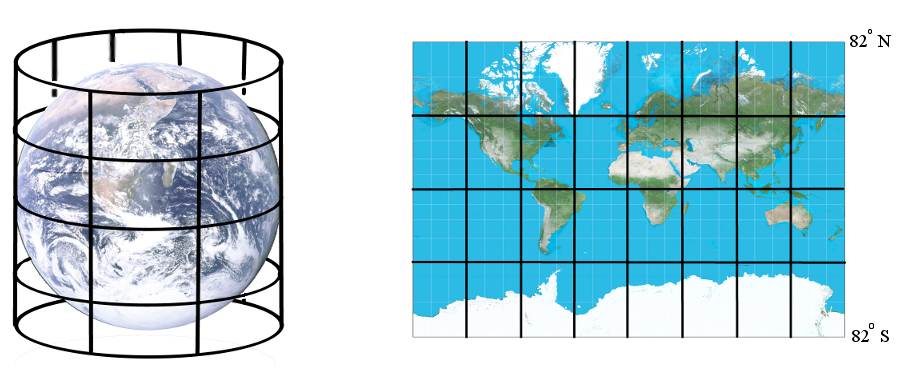
\includegraphics[scale=1.8]{./images/Mercator.jpg}
\caption[Scott Hotton's modification of an image from the Cartographic Research Lab at the University of Alabama.]{The Earth's surface in 3 dimensional space is rendered as a flat, 2
dimensional surface by the Mercator projection method. Most of the distortion
produced by the projection occurs near the Earth's poles so small regions 
around the poles are cropped out from the maps. Most of the continents and
oceans undergo little distortion by the projection which made it a popular 
projection method for making maps of the Earth.} 
\label{Mercator}
\end{figure}
% From https://upload.wikimedia.org/wikipedia/commons/9/97/The_Earth_seen_from_Apollo_17.jpg  AND https://upload.wikimedia.org/wikipedia/commons/f/f4/Mercator_projection_SW.jpg
% Possibly redraw


% The Mercator projection maps the Earth's surace to an infinite strip. It is
% not a radial projection from the center of the Earth, through the Earth, to
% the surrounding cylinder. There are websites that say otherwise but they are wrong.

% For next pass (jeff). Topology is preserved. Distances are not (see Greenland). Abstractly: topology is preserved, but not the metric.

   We can still use the projection to get a sense of the layout of the Earth. 
How are we able to do this?  One reason is that certain {\em topological} 
properties of the Earth's surface--that is, properties involving 
continuity--are preserved by the projection. For example, when we see on the 
map that Los Angeles and San Francisco are on the same coast, then we know we 
can sail along the coast to get from one city to the other. San Francisco is
closer to Merced than it is to Los Angeles, but when we see on the map that 
Merced is not on the coast, then we know that we can not sail from San Francisco 
to Merced. Even though distances on the map have been distorted slightly we 
can still use it to make travel plans. 

% (Jeff notes) Example of spherical pendulum is (almost) a Foucault's penduluum. Like at the observatory. Hanging bob constrained to be on surface of a sphere. Physically familiar. 2 angular coordinates (like lines of latitude and longitude) and 2 velocity coordinates. (Compare regular planar penduluum: circle times line for velocities = tangent bundle for a circle. So 2 dimensional). This 4d thing is tangent  bundle to S2 (which is not S2 x R2). So basically a complex thing that�hard to visualize, since it's not a cartesian product. There is no simple thing to compare it to. // Examples shown is a single surface that contains orbit that maintain the same energy and engular momentum. // Intersection of a level set of the energy function and a level set of the  angular momentum function. //   MAYBE DO IT THIS WAY. Higher dimensional object can't be visualized. We don't know what kind of surface it is. Oh look we can project it to a lower division and see it looks like a torus and is symmetrical. This is a real example that was used in practice. An example of a projection that was actually usefulin practice. A real world example. It did not solve a problem without a solution, but it helped communicate the solution to people who might not otherwise understand the paper. It helps mathematicians understand things that are hard to  understand otherwise. (Ask Scott more about what was revealed.)

   We can use the method of projection to visualize even higher dimensional 
spaces that can not be seen by human eyes. A somewhat exotic example is shown 
on the right of figure \ref{F:projection}. This is the projection of a 2 
dimensional surface in a 4 dimensional space down to a 3 dimensional space. 
The 4 dimensional space is the state space for a spherical pendulum, and the 
surface is the set of all states of the pendulum that have the same energy and 
angular momentum. We can see it resembles the surface of a donut with a groove
along the side. 

   Another example is shown on the left of figure \ref{F:projection}. It 
consists of three circles that intersect at a single point (called a ``bouquet 
of three circles''). In this example, the three circles are perfectly round and 
lie in three mutually perpendicular planes, but we can not see this bouquet of 
circles directly with our eyes. We also can not see, directly with our eyes, 
that this bouquet of circles forms a symmetrical figure in a 6 dimensional 
space. Although the projection distorts the figure a little and we lose some 
of the roundness of the circles in the projected image, we can still see the 
symmetry of the overall figure. The software that was used to do this 
projection is part of Simbrain (the ``projection plot''). This plot can be 
used to visualize structures in the higher dimensional spaces associated with 
many neural networks.

\begin{figure}[h]
\centering
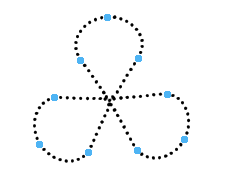
\includegraphics[scale=2.7]{./images/Sammon3.png}
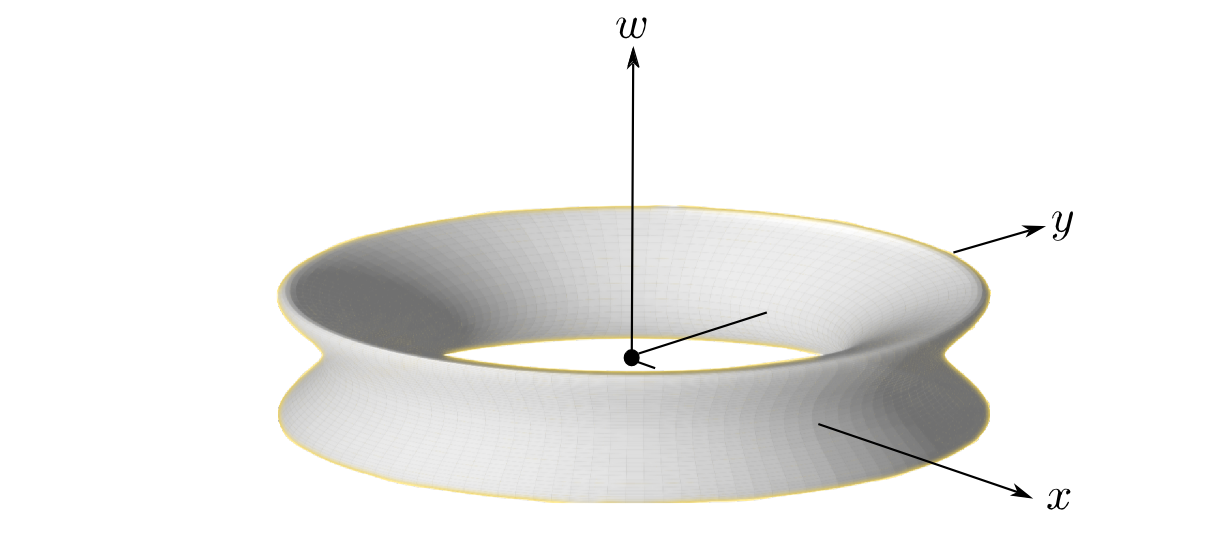
\includegraphics[scale=0.22]{./images/torus.png}
\caption[Scott Hotton.]{(Left) The projection of a symmetrical curve in a 6 dimensional space 
so that we can see its symmetry. The nine vectors listed at the beginning of 
section \ref{S:dimred} are shown as nine large blue dots. (Right) A 
symmetrical surface in a 4 dimensional space is projected so that we can see 
its symmetry.}
\label{F:projection}
\end{figure}

There are many different methods for projecting data from high dimensional spaces to lower dimensional spaces, and the field as a whole is called ``dimensionality reduction''. Each projection method has its pros and cons, and each one introduces different forms of distortion. But by using several such projections one can often get a good sense of the structure of some high dimensional data.\footnote{The three methods used in Simbrain are described here: \url{http://hisee.sourceforge.net/about.html}. Other methods of projection are available in this free Matlab toolbox: \url{http://homepage.tudelft.nl/19j49/Matlab_Toolbox_for_Dimensionality_Reduction.html}.}

\section{The Dot Product}\label{dotProduct}

% Nice visualization: http://www.falstad.com/dotproduct/
% Include discussion of orthogonality and closeness from NeuralNets.txt
% If we are doing "distance" on a unit hypersphere, then the dot product  is really an inverse metric. max is 1 then as you go to -1 it is increasingly far away (See that falstad applet to show this).
% The negative cases are important when thinking of a weight vector as orthogonal to a decision boundary  in a network with threshold units

 The \glossary{dot product} is a simple but important function defined 
for pairs of vectors in a vector space.\footnote{The dot product is more 
formally known as the ``scalar product.'' The scalar product gets its name from 
the fact that its value is a scalar. The scalar product is a member 
of a general class of functions known as ``inner products''. Inner products 
are used to express geometric relationships between vectors.}  The dot 
product is different from scalar multiplication (scalar multiplication and the 
scalar product are defined in section \ref{S:LinearAlgebraAppendix}). The dot 
product is a function of two vectors, whereas scalar multiplication is a 
function of a vector and a scalar. The dot product gets its name from the fact 
it is represented by a large dot: $\bullet$. It is also common to say that we 
are ``dotting'' one vector with another.
\begin{figure}[h]
\centering
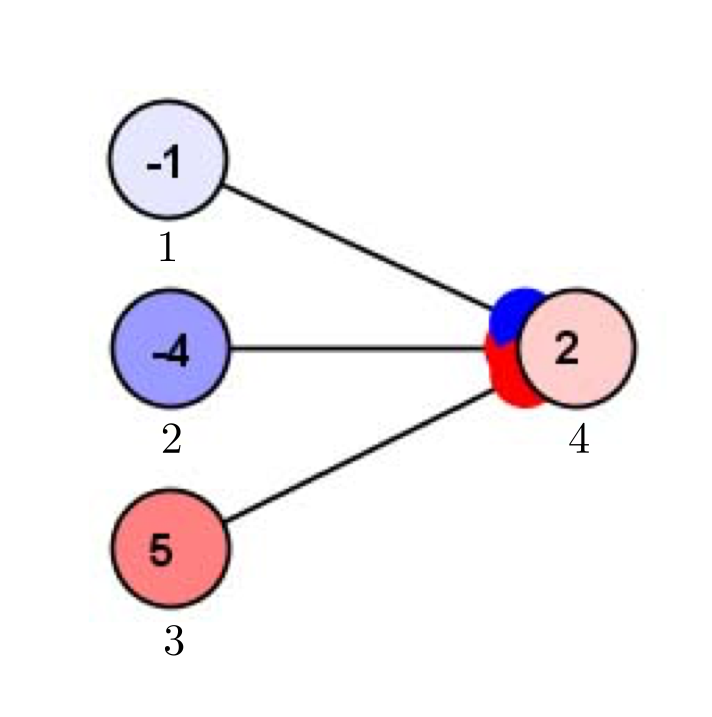
\includegraphics[scale=.7]{./images/Simple3Labelled.png}
\caption[Simbrain screenshot.]{Simple feed-forward network with nodes labeled. The dot product can be used to compute the weighted inputs to node 4.}
\label{F:simplelabelled}
\end{figure}

   The dot product is computed by multiplying each of the corresponding 
components of a pair vectors, and summing the resulting products. For example
\begin{eqnarray*}
&(1,2,3)  \bullet  (4,5,6)& = \quad 1 \cdot 4 + 2 \cdot 5 + 3 \cdot 6 = 32   \\
&(0,0,0)  \bullet  (4,5,6)& = \quad 0 \cdot 4 + 0 \cdot 5 + 0 \cdot 6 = 0    \\
&(2,3,-1) \bullet (-1,1,1)& = \quad 2 \cdot (-1) + 3 \cdot 1 + (-1) \cdot 1 = 0 \\
 &(1,1,1,1,1) \bullet (1,1,1,1,1)& = \quad  
          1 \cdot 1 + 1 \cdot 1 +  1 \cdot 1 + 1 \cdot 1 + 1 \cdot 1 = 5
\end{eqnarray*}

   Clearly the product of any vector with the zero vector (the vector whose
components are all $0$) is $0$. However, the dot product of two non-zero 
vectors can also be $0$. It turns out that if the dot product of two non-zero 
vectors is $0$, then the vectors are {\em orthogonal} (perpendicular) to each 
other. It might be hard to tell right away that the vectors 
$(2,-1,1,-3,1,1)$, $(1,2,3,1,1,-1)$ are orthogonal to each other, but a quick calculation 
shows us
\begin{eqnarray*}
 (2,-1,1,-3,1,1) \bullet (1,2,3,1,1,-1)& = 0
\end{eqnarray*}
so they must be orthogonal. 
%The dot product can also be used to uncover other geometric properties in high dimensional spaces.

 Notice that we can concisely represent the weighted input (see chapter \extref{ch_act_functions})
to a node using the dot product. The weighted input is just the dot product of
the activation vector with the fan-in weight vector of the output node, plus a
bias term. For example, if the weight vector for node $4$ in figure \ref{F:simplelabelled} is 
$(-1,-1,1)$, then the net-input is
\begin{equation*}
n_4 = (\; -1,\; -4,\; 5) \bullet (-1,-1,1) + 0  = 1 + 4 + 5 + 0 = 10
\end{equation*}


% For example, we can describe the weighted input to node $k$ (as $k$ goes
%from $1$ to $m$) as follows:
%\begin{equation*}
%n_k = (w_{1,n},w_{2,n}, \dots, w_{m,n}) \bullet (a_1,a_2, \dots ,a_m) + b_n
%\end{equation*}

% dot(u,v) = u*v
% cos_sim(u,v) = u*v/|u|*|v|, which happens to also be cos(theta btween u and).
%			i.e like dot by divide by magnitude of u and v
% cov(u,v) = like dot but subtract out mean
% corr(u,v) = like cov but divide magnitude of u and v


% Expand to include a broader discussion that includes cosine similarity 
%      - Dot product: not scaled, not centered.
%      - Cosine similarity: scaled, not centered
%      - Covariance: centered, not scaled
%      - Correlation: scaled and centered 

% These operations don't really apply to pairs of numbers (except trivially), but rather to pairs of vectors

% Different ways the data tend to be gathered
% smell vector 1 = (1,1,1,0)
% smell vector 2 = (1,1,1,0)
%
% weight/height
% human 1  		= (5, 120)
% human 2  		= (5.5,180)
% human 3  		= (6.5,210)

%% Email from Scott:  I said a while ago that i would get back to you on cosine simarlity and
%the Pearson correlation coefficient.  I think the cosine similarity statistic
%is used when the things being compared have the same units of measure.
%
%  The Pearson correlation coefficient is the cosine similarity of the data 
%after it has been centered.
%
%  To center data (x1, ..., xn) we subtract their mean from each entry.
%
%                ( x1, ..., xn) -> ( x1-xbar, ..., xn-xbar) 
%
%Geometrically the centered data is the orthogonal projection of (x1, ..., xn) 
%to the subspace orthogonal to the vector (1, ..., 1).  This subspace has 
%dimension n-1.  The projection can reduce the angle between two vectors (x1, 
%..., xn) and (y1, ..., yn).  In a sense there are fewer ways they can 
%point away from each other when we reduce the number of dimensions by 1.
%
%  By centering the data before taking the cosine similarity we avoid 
%spurious differences introduced by the choice of units of measure.  Both 
%(x1, ..., xn) and (y1, ..., yn) are thought of as vectors in R^n but the 
%n-tuples of numbers can stand for different quantities.  For instance we could 
%measure the germination time of seeds as a function of temperature.  If we 
%measure temperature in Celsius and time in seconds we will get a different 
%cosine similarity than if we measure temperature in Celsius and time in hours.  
%Whereas the Pearson correlation coefficient will be the same either way.
%
%  In a case like in the Wikipedia article which involves comparing the words
%in two documents there are not two different units of measure for the two 
%things being compared.  Not centering the data may have little effect on the 
%usefulness of the statistic in this case but it could save computation time. 

%The normalized dot product between two vectors, also known as the cosine similarity, calculates the angle between two vectors such that the similarity calculation is not impacted by magnitude. Bounded between $[-1, 1]$, such that $\cos = -1$ indicates opposite vectors, $\cos = 0$ indicates orthogonal vectors, and $\cos = 1$ are proportional vectors. Some implementations are bounded between $[0,1]$. Occasionally, cosine distance is used, which is $1 - \cos$, in which case proportional or highly similar vectors will have a cosine distance of 0, while dissimilar vectors will have a cosine distance of 1.
% Add some exercises to the end.


\section{Vector Spaces as Metric Spaces}

A vector space can have a metric, which is a way to define the distance between any two points. The usual metric for a real vector space is the Euclidean metric, which can be expressed in terms of the dot product. The Euclidean metric uses the concept of a norm, denoted by double bars $|| \cdot ||$, which measures the ``length'' of a vector. Specifically, the norm of a vector $\mathbf{x}$ is the square root of the dot product of the vector with itself: $||\mathbf{x}|| = \sqrt{\mathbf{x} \bullet \mathbf{x}}$.  With this
metric the distance between any pair of vectors in $\real^n$ is:
\begin{equation*}
\mathbf{x} = (x_1, x_2, \ldots, x_n) \qquad
\mathbf{y} = (y_1, y_2, \ldots, y_n) \qquad
\end{equation*}
is:
\begin{equation*}
|| \mathbf{x} - \mathbf{y} || =
\sqrt{ (\mathbf{x} - \mathbf{y}) \bullet (\mathbf{x} - \mathbf{y}) }
= \sqrt{ \sum_{j=0}^n (x_j - y_j)^2 }
\end{equation*}
There are many metrics for every vector space but usually we use the Euclidean metric.

% Consider adding a plot showing nearby points here.
The upshot of this is that we can interpret the vector spaces associated with neural networks--activation spaces, input spaces, weight spaces, etc.--as giving us a sense of how far apart relevant vectors are, and thus how similar the things they represent are. Points nearby one another in an input space correspond to similar inputs: similar smells, similar visual inputs, similar words relative to a word embedding (chapter \extref{ch_word_embeddings}), etc. Points nearby one another in a weight space are similar configurations of weights. These interpretations are often emphasized in analyses of neural networks (for example, see chapter \extref{ch_representations}), and in fact the spaces associated with neural networks are sometimes called ``similarity spaces''.  An example which illustrates the importance of this way of thinking is figure \extref{competitiveInputSpace}.

\section{Matrices}\label{sect_matrices}

% Officially stipulate our usage: components of a vectors, entries of a matrix.

   Another object studied in linear algebra is a \glossary{matrix}, which is a 
rectangular array of numbers arranged into rows and columns: basically a table of 
values. Here is an example of a matrix:
\[
\begin{pmatrix}
 1  &   9  & 7 \\
 5  &   3  & 2 \\
0.3 &  -1  & 0 \\
 0  & -0.4 & 0
\end{pmatrix}
\]
It is conventional to describe matrices by stating the number of rows and 
columns they have, in that order. The example above is a $4 \times 3$ 
matrix because it has 4 rows and 3 columns.\footnote{The notation for vectors typically includes a comma-separated list of the vector's components. The notation for matrices typically does contain not commas. A  matrix's components are only aligned into rows and columns without any extra characters to separate them. Otherwise we think of vectors as special cases of matrices. A vector with $n$ components can be represented as either a $1 \times n$ matrix or as an $n \times 1$ matrix. So far we have been representing vectors as $1 \times n$ matrices.}  Each row of a matrix is called a \glossary{row vector} and each column is called a \glossary{column vector}. The matrix above has four row vectors and 
three column vectors.\footnote{Note that vectors  are matrices and matrices are vectors!  As already noted, vectors are a special kind of a matrix, 
a matrix with one row or one column. Conversely, matrices are technically a 
kind of vector, since they satisfy the formal definition of a vector (they 
exist in vector spaces called ``matrix spaces''). However, it will be easier for us to follow standard practice and treat these as separate kinds of mathematical objects.}

\begin{figure}[h]
\centering
\raisebox{-0.5\height}{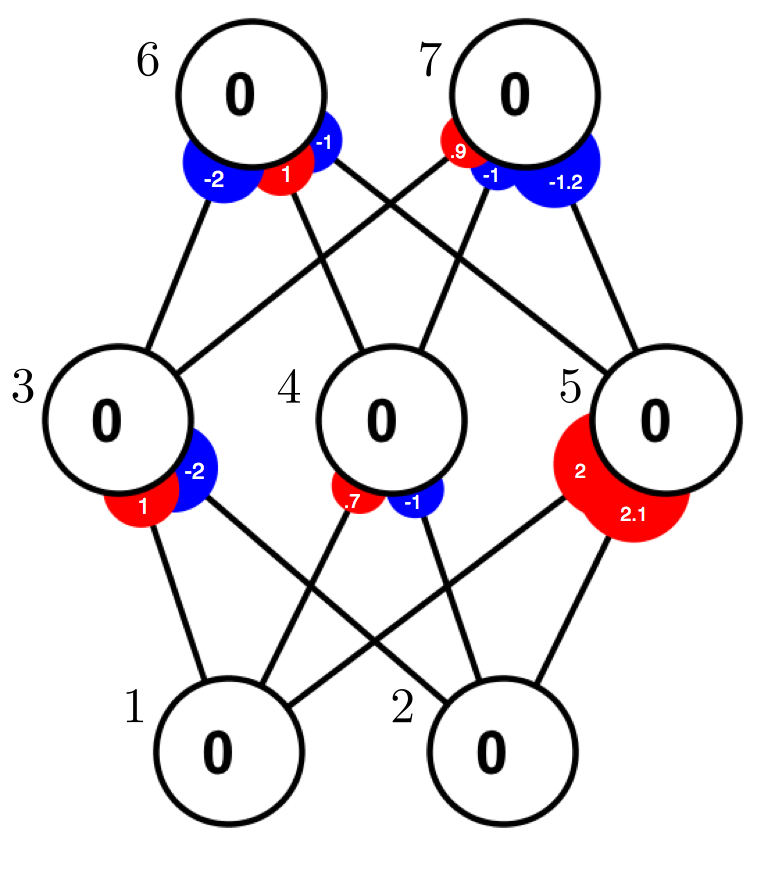
\includegraphics[scale=.45]{./images/ff_labelled.png}}
\hspace*{.7in}
\raisebox{-0.5\height}{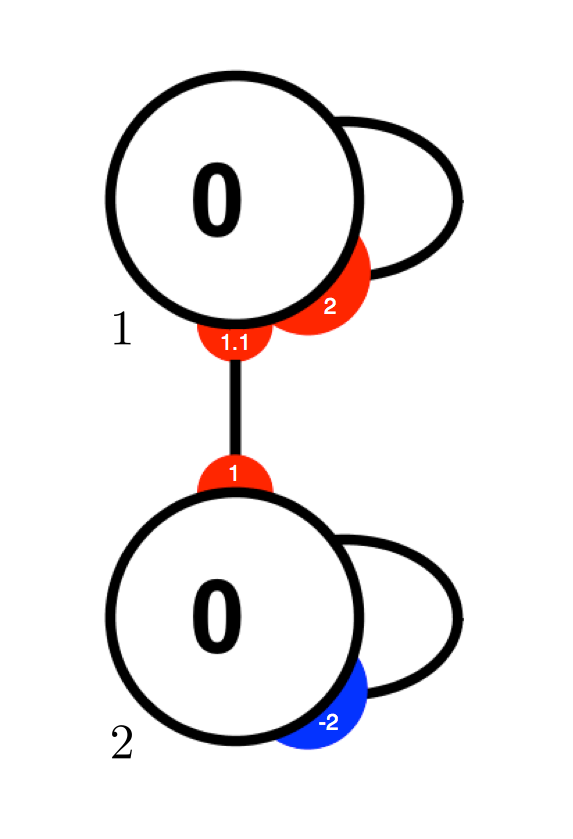
\includegraphics[scale=.2]{./images/recurrent_labelled.png}}
\caption[Simbrain screenshots modified by Jeff Yoshimi.]{Feedforward and recurrent networks with nodes labelled, and weight strengths shown. Each weight layer of the feedforward network and the weights of the recurrent network can be associated with weight matrices. }
\label{labelledNets}
\end{figure}

We adopt the convention of writing matrices using bold-faced upper-case letters, for example $\mathbf{W}$ or $\mathbf{R}$. By contrast, non bold-faced, italic lower-case letters are reserved for entries in a matrix, and subscripts indicate which row and column. For example $w_{2,3}$ could be the scalar at the second row and third column of a $2 \times 3$ matrix $\mathbf{W}$.\footnote{In physics and mathematics it would be more conventional to use upper-case letters like $W_{2,3}$ of the matrix $\mathbf{W}$ for this purpose, but we here follow more standard conventions in discussions of neural networks.} In the matrix above, for example, $w_{1,3} = 7 $

\section{Weight Matrices}

Matrices are often used to represent the weights of a network. This facilitates a compact way of describing many of the computations involved in updating a neural network. The weights of a neural network can be represented by a matrix by labeling the rows and columns of a neural network with indices $1,\dots,n$ for rows, and $1,\dots,m$ for columns. Then we can represent the strength of a weight from node $j$ to node $k$ as the value in the $j^{th}$ row and $k^{th}$ column of a weight matrix.\footnote{\label{sourceTarget} This can be called a ``source-target'' representation, because rows are associated with source neurons and columns are associated with target neurons. Some neural network texts (especially older ones) use a ``target-source'' representation, where rows are associated with target neurons and columns are associated with source neurons.} This implies that a source-target weight matrix representation of a set of weights will have as many rows as source neurons and as many columns as target neurons.

We first consider weight layers in feedforward networks. Each weight layer of a feedforward network can be represented by its own weight matrix $\textbf{W}_{i,j}$ where $i$ is the source node layer and $j$ is the target layer. For example, $\textbf{W}_{1,2}$ or $\textbf{W}_{input,hidden}$ is the matrix connecting the input node layer to the hidden node layer on the left of figure \ref{labelledNets}. The column and row headings are shown in bold text and match the node labels in \ref{labelledNets}. Notice that there are as many rows as input neurons and as many columns as hidden layer neurons. You can see, for example, that the weight $w_{2,4}$ from node 2 in the input layer to node 4 in the weight layer is in the row labeled 2 and the column labeled 4: -1. On the right is a more standard matrix representation of $\textbf{W}_{1,2}$.

\begin{minipage}{0.5\textwidth}
\centering
\[
\begin{array}{|c|c|c|c|}
\hline
\multicolumn{1}{|c|}{} & \textbf{3} & \textbf{4} & \textbf{5} \\
\hline
\textbf{1} & 1 & 0.7 & 2 \\
\hline
\textbf{2} & -2 & -1 & 2.1 \\
\hline
\end{array}
\]
\end{minipage}
\begin{minipage}{0.5\textwidth}
\centering
\[
\begin{pmatrix}
1 & 0.7 & 2 \\
-2 & -1 & 2.1 \\
\end{pmatrix}
\]
\end{minipage}
\vspace*{.1cm} 

\noindent Notice that columns of the weight matrix correspond to fan-in weight vectors for the hidden layer (rows correspond to fan-out). This implies that you can compute weighted inputs at the hidden layer by the dot product of an input vector and each column, a topic we discuss next. Regardless convince yourself you can see the link between fan-in weight vectors and columns. 

As an exercise, see if you can produce the weight matrix representation for $\textbf{W}_{2,3}$ or $\textbf{W}_{hidden,output}$. Hint: it has 3 rows and 2 columns. 

Now the recurrent case, starting with the recurrent network shown in figure \ref{labelledNets}. Here the source and target neurons are the same and so the weight matrix, which we can call $\textbf{W}_{recurrent}$, is square: it has as many rows as columns. To fill it out we follow the same procedure, going from source label to target label and finding the corresponding entry. For example, $w_{1,2}$ is the weight from node 1 to 2, and is thus in the first row, second column of the matrix. Confirm the values match up:

\begin{minipage}{0.5\textwidth}
\centering
\[
\begin{array}{|c|c|c|}
\hline
\multicolumn{1}{|c|}{} & \textbf{1} & \textbf{2} \\
\hline
\textbf{1} & 2 & -.5 \\
\hline
\textbf{2} & -1 & 1.2 \\
\hline
\end{array}
\]
\end{minipage}
\begin{minipage}{0.5\textwidth}
\centering
\[
\begin{pmatrix}
 2  &  -.5 \\
 -1  & 1.2 
\end{pmatrix}
\]
\end{minipage}
\vspace*{.1cm} 

\noindent In a weight matrix for a recurrent network diagonal entries correspond to connections from a node back to itself. Also note that fan-in weight vectors still correspond to columns. The first node has fan-in weights of -2 and 1, the second has fan-in weights of .5 and 1.2.

\begin{figure}[h]
\centering
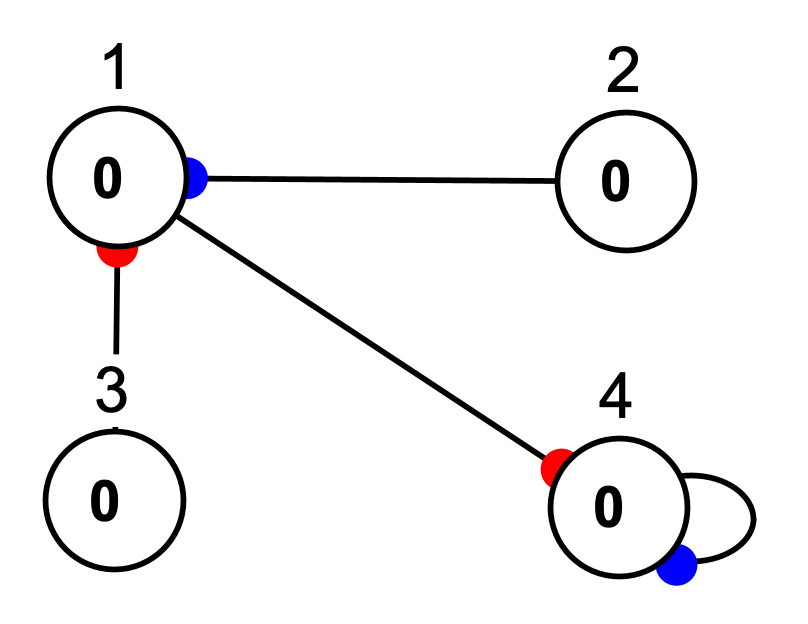
\includegraphics[scale=0.5]{./images/sparseRecurrent.png}
\caption[Jeff Yoshimi.]{A sparse recurrent network, where most of the possible connections do not exist, so that in its matrix representation most entries will be 0. In this network red weights have a strength of 1 and blue weights have a strength of -1.} 
\label{sparseRecurrent}
\end{figure}

Figure \ref{sparseRecurrent} shows another example, that shows what we do when some links are missing. If a weight does not exist, it is represented by a $0$ in the corresponding matrix. Here is its representation:

% Make this a table with a caption but keep this position
\begin{minipage}{0.5\textwidth}
\centering
\[
\begin{array}{|c|c|c|c|c|}
\hline
\multicolumn{1}{|c|}{} & \textbf{1} & \textbf{2}  & \textbf{3} & \textbf{4} \\
\hline
\textbf{1} & 0 & 0 & 0 & 1 \\
\hline
\textbf{2} & -1 & 0 & 0 & 0 \\
\hline
\textbf{3} & 1 & 0 & 0 & 0 \\
\hline
\textbf{4} & 0 & 0 & 0 & -1 \\
\hline
\end{array}
\]
\end{minipage}
\begin{minipage}{0.5\textwidth}
\centering
\[
\begin{pmatrix}
0 & 0 & 0 & 1 \\
-1 & 0 & 0 & 0 \\
1 & 0 & 0 & 0 \\
0 & 0 & 0 & -1
\end{pmatrix}
\]
\end{minipage}
\vspace*{.1cm} 

\noindent Now let's check your understanding: there are 4 nodes and thus the matrix is 4-by-4. There are two positive weights and two negative weights, and there are two positive entries and two negative entries in the table. Node 4 is self-connected and the fourth diagonal entry is non-zero. Nodes 1 and 4 have two weights in their fan-in and those two columns have two entries.

% Change refs below to refs to the table
In the special case where most of the entries in a weight matrix are $0$, the matrix is called a \glossary{sparse matrix}. The matrix representing the weights in figure \ref{sparseRecurrent} is sparse. A sparse matrix is contrasted with dense matrix, where most of the entries are non-zero. Really these are two ends of a continuum described by a number called \glossary{sparsity}, which ranges from $0$ to $1$, and where higher values are more sparse. The sparsity of a matrix is obtained by counting how many zero entries the matrix has and dividing by the total number of entries. If all of the matrix entries are $0$ then the sparsity of the matrix is $1$. If half of the entries are $0$ then the sparsity is $.5$.  If none of the matrix entries are $0$ then the sparsity of the matrix is $0$. The matrix in the table above has $16$ entries, $12$ of which are $0$, so its sparsity is $12/16 = 3/4 = .75$. Sparse weight matrices represent sparsely connected networks, where only a few of the possible connections between relevant nodes exist (recall that a matrix representation of a network uses $0$ to represent the absence of a connection).  Dense matrices are used to represent densely connected networks. The word ``dense connection'' or ``dense weight layer'' in this context often implies a sparsity of $0$, that is, an ``all-to-all'' or ``fully connected'' set of weights between relevant nodes.
% Think about whether some clarification about feed-forward and recurrent weight layers is needed

\section{Vector-Matrix Product}

% TODO: Should obviously update this material once the new material is added
The power of matrices in neural networks is our ability to use them to represent weights and transformations of activation vectors as they propagate. We are splitting the topic into two parts. For the version of the course the book currently focuses on, we only consider one case: a vector-matrix product. We can understand this in a simplified way using mainly just the dot product. But this is just a specially curated case, and the full story is more complex and involves more cases.\footnote{\label{leftRightConvention}  We will not give a general definition of matrix multiplication or matrix product here. Instead, we will describe a special case of it: ``vector-matrix'' multiplication, which involves multiplying an activation vector on the left times a weight matrix on the right.We are presenting the computation as a row vector on the left times a weight matrix on the right, which is required by the ``source-target'' representation (see note \ref{sourceTarget}). It is also easy to think about in terms of the operations involved in updating a neural network: an activation vector is ``passed through'' a weight matrix to produce another activation vector, in this case a hidden unit vector. However, this is non-standard. In linear algebra and most applications this operation would usually be represented with the matrix on the left and a column vector on the right. This is because a matrix is often thought of as a function that operates or acts on a vector, transforming inputs to outputs.}  But we're starting simple.

So the way we do things here, we focus on taking an input vector, and dotting it with columns of a weight matrix, which (in the source-target format) represent fan-in weight vectors. In this way we produce a new output vector. Each of these dot products is a weighted input (see chapter \extref{ch_act_functions}). Assuming a default unbounded linear activation function, this can be used to represent weight propagation. We consider the feed-forward case first, then the recurrent case.

Feed-forward. Consider the feed-forward network in figure \ref{labelledNets}, which uses linear activation functions without bias (we are also ignoring clipping) so that node activations just are weighted inputs. That is, we multiply the input vector by the intervening weight matrix to obtain the hidden unit vector:  $\textbf{a}_{hidden} = \textbf{a}_{input} \textbf{W}_{input,hidden}$. We can then multiply the hidden unit vector by the hidden-to-output layer weight matrix to get the output vector. We can continue to do this for all the layers of a feed-forward network. So, for linear networks, pretty much all we do when updating the network is use matrix products (and even for non-linear networks, we use the matrix product to compute vectors of weighted inputs, which are then transformed by, for example, sigmoid functions).

Here is an informal description of how to multiply a vector on the left by a matrix on the right: take the dot product of the vector on the left and the first column vector in the matrix. The resulting number is the first component of a row vector, which will be the result of this operation. Then do this for each of the remaining columns of the matrix, adding these dot products to the row vector as you go. The resulting row vector is the matrix product of a row vector and a matrix. Intuitively, it is like you are writing out the matrix product, one number at a time, by dotting the vector on the right with each of the columns of the weight matrix.

Consider an example. Suppose the feed-forward network in figure \ref{labelledNets} has linear activation functions and 0 bias, and its input activation vector is $\textbf{a}_{input} = (1,2)$. To compute the hidden layer activation vector, we compute the dot product between the input vector and each of the three column vectors:
\[
  \begin{matrix}\begin{pmatrix}1 & 2\end{pmatrix}\\\mbox{}\end{matrix}
  \begin{pmatrix} 1 & 0.7 & 2 \\ -2 & -1 & 2.1 \end{pmatrix} 
  =
  \bigg( (1)(1) + (2)(-2) ,\;\; (1)(0.7) + (2)(-1) ,\;\; (1)(2)+ (2)(2.1) \bigg)
  =
  \begin{pmatrix}  -3 \;\; -1.3 \;\;\; 6.2  \end{pmatrix}
\]
\vspace*{.1cm} 

This can be visualized by imagining that an input activation vector is being combined (``dotted'') with the fan-in weight vectors of each of the three nodes at the next layer, to produce the weighted input to each of them and thus the next layer's activation vector. 

% 1,2 as input confusing because it overlaps indices in video. Change?
Now for the recurrent case. We can do the same kind of thing with the sparse recurrent network in figure \ref{sparseRecurrent}, but in this case we will be determining its activations at successive time steps. This is because with a recurrent network, the output can always be fed right back into the network as input, which gives these networks their dynamic properties. Let the weight matrix be  $\textbf{W}_{r}$ then a sequence of activation vectors $\textbf{a}(1), \textbf{a}(2), \textbf{a}(3), \dots$ (with time in parentheses) is given by $\textbf{a}(2) = \textbf{a}(1) \textbf{W}_{r}$, $\textbf{a}(3) = \textbf{a}(2) \textbf{W}_{r}$, etc. 

This is easy to see by exmaples. Suppose we have activated node 2 of the network in figure \ref{sparseRecurrent} and we start iterating. Since the activations and weights are all whole numbers, it's not too hard to compute this out for a few time steps. Again just dot the input vector by the columns to write out the first output, where we get the activation vector at time 2 by multiplying the initial activation vector by the weight matrix (that is, $\textbf{a}(1) \textbf{W}_{r} = \textbf{a}(2)$):
\[
\begin{pmatrix}
0 & 1 & 0 & 0  
\end{pmatrix} 
\begin{pmatrix}
0 & 0 & 0 & 1 \\
-1 & 0 & 0 & 0 \\
1 & 0 & 0 & 0 \\
0 & 0 & 0 & -1
\end{pmatrix}
=
\begin{pmatrix}
-1 & 0 & 0 & 0
\end{pmatrix} 
\]
\vspace*{.1cm} 

\noindent Try to do it in your head, dotting the $(-1, 0,0,0)$ with the four columns of the matrix and thereby writing out the output vector. In the next iteration you will get $(0,0,0,-1)$, then $(0,0,0,1)$. If we keep going we get the following sequence of states from the initial state $(0,1,0,0$):
\begin{equation*}
(0,1,0,0),\; (-1,0,0,0),\; (0,0,0,-1),\; (0,0,0,1),\;  (0,0,0,-1)\; \dots
\end{equation*}
You can easily set this up in Simbrain and confirm this is what happens. We will see in the dynamical systems chapter \extref{ch_dst} that this is one \emph{orbit} in the network's activation space. In this case, the network has started to oscillate between two states, and it will do that forever, and that behavior is basically encoded in the weight matrix.
 
%The idea that a matrix represents a way of transforming vectors is common in mathematics. In fact, matrices are often used to represent linear transformations, where one vector is converted in to another using a linear function. Think of a set of points in the plane (vectors in a 2 dimensional space) getting moved in some specific way. The way these points move can be represented, in some cases, by multiplying each point by a matrix. For example, when you use a drawing program to modify a simple line graphic (a bunch of points in a plane) the transformation of the selected set of points is implemented using matrix multiplication. Rotations about the origin, reflections about a line through the origin, and dilations and contractions about the origin are linear transformations.

\section{Tensors}\label{sect_tensors}

% https://stanford.edu/~shervine/teaching/cs-230/cheatsheet-convolutional-neural-networks

A \glossary{tensor} is a generalization of the concept of a vector that encompasses numbers, arrays of numbers, matrices (2d arrays of numbers), arrays of matrices, arrays of these arrays, etc. These more complex structures are increasingly common since the time of the deep learning revolution (section \extref{deep_revolution}). The basic idea is not just to work with vectors and matrices, but also sets of matrices and even sets of sets of matrices. These have special nomenclature like ``volume''. In this section we cover the basics.

% TODO: Glossary items for textbfs
% Array vs. set.  Array implies ordering. Comp sci version of tuple.
% Tensor is more math language. Ndarray is more from languages like numpy and torch
The \textbf{rank} of a  tensor is the number of indices required to specify an entry in it.These are also sometimes called ``n-dimensional arrays'' or ``n-d arrays'' (1d array, 2d array, etc.).\footnote{Note that the dimensionalty of an array is the literal dimension of the object, like a vector is 1d and a matrix is 2d. This is not the same as the dimensionality of the space these objects live in. For example, $(1,2,1,0)$ is a point in a 4d space, but it is a 1d tensor or 1d array of numbers.} The \textbf{shape} of a tensor is the number of components it has along each of the array's dimensions. We have seen this with matrices, where the shape is stated in terms of rows and columns, e.g. a $5 \times 2$ matrix. For more complex tensors the shape is specified by a number of components for each dimension of the array, like a $4 \times 2 \times 5$ volume. Here are the main types of tensor:

\begin{itemize}
\item A \textbf{scalar} is a rank 0 tensor or 0d array because it requires no indices. The number 42 is a rank 0 tensor, a 0d array, but nobody talks about it that way. 
\item A \textbf{vector} is a rank 1 tensor or 1d array because it takes one index to specify an entry in a vector, and the result is spread out in one dimension. The vector $(0,1,0)$ is a rank 1 tensor, because it takes one index to specify entries, but people usually just call it a vector. Vectors were discussed in much of this chapter, starting in section \ref{sect_vector}.
\item A \textbf{matrix} is a rank 2 tensor or 2d array, because it takes two numbers to specify an entry (a row and column index), and the result is spread out in two dimensions. We've seen lots of examples of matrices in this chapter, and they were discussed in section \ref{sect_matrices}.
\item A \textbf{volume} is an array of matrices. It is a rank 3 tensor or 3d array, because it takes 3 indices to specify an entry, and the result is spread out in three dimensions. The term ``volume'' is common but not completely standard, but is intuitive so we adopt it here. It can be visualized as a stack of matrices, or as a solid, something like a Rubik's cube or 3d chess board (see figure \ref{tensorVisualStyles}). A common use of volumes is to represent images, which requires several channels of 2d information, several ``copies'' of a pixel array. For example, an RGB color image that is 28 rows (height) by 28 columns (width) is represented by three matrices (red, green, and blue) of shape $28 \times 28$. Thus the whole image is represented by a tensor with shape $3 \times 28 \times 28$.  These indices are referred to as channel, width, and height. 
\item A \textbf{batch of volumes} is an array of volumes. It is a rank 4 tensor or 4d array because it takes 4 indices to specify an entry. It is spread out in four dimensions, but since we can't visualize that we can instead visualize a set of volumes, as in the right panel of figure \ref{tensorTypes}. The word ``batch'' is used here because we are often dealing with sets or batches of inputs in a training dataset (see chapter \extref{ch_data_science}), in this case batches of RGB images, each of which is a volume with 3 channels. For example, if the images are $3 \times 28 \times 28$, then the batch of 100 images has shape $100 \times 3 \times 28 \times 28$. 
\end{itemize}

 % Rank 5 tensor examples: batch size x time steps x height x width x channels. Brain scan. Each brain scan is 3d and it's color so there are channels. So a batch of those.

Examples of each of these types of tensor are shown in figure \ref{tensorTypes}. More examples are in chapter \extref{ch_cnn}.

\begin{figure}[h]
\centering
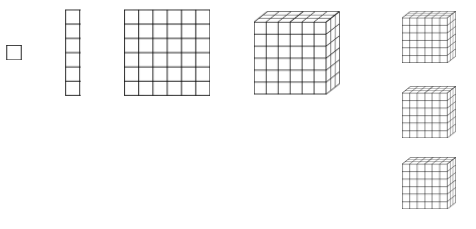
\includegraphics[scale=0.6]{./images/tensorTypes.png}
\caption[Soraya Boza.]{Schematic of different types of tensor. From left to right: a scalar, a vector, a matrix, a volume, and a batch of volumes. It can be seen that they are 0d, 1d, 2d, 3d and 4d arrays.  Numbers are not drawn in; only the abstract shape of the tensors are shown.} 
\label{tensorTypes}
\end{figure}

\begin{figure}[h]
\centering
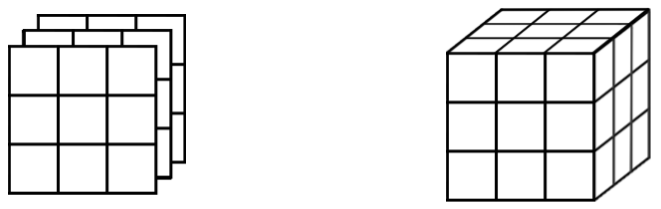
\includegraphics[scale=0.3]{./images/tensorVisualStyles.png}
\caption[Soraya Boza.]{Two ways a representing a 3d array: a stack of matrices (left) vs. a solid ``Rubik's cube''  or volume (right). Depending on the context one or the other representation is more useful.} 
\label{tensorVisualStyles}
\end{figure}

We can refer to the different indices for a tensor using standardized names in a standard order: batch size, depth (number of channels), height, and width.\footnote{This is sometimes called NCHW format (number of samples, channels, height, width). However, usage varies. Some put height and width first in indexing; some put them last in indexing. Even though the rank of a tensor is the number of indices \emph{required} to specify an entry, sometimes additional entries are included (e.g. specifying a vector as a column vector assumes it is being placed in a 2d space). Thus the presentation of the ``shape'' of a tensor can vary.  In figure \ref{tensorTypes} the shapes might be given as $1 \times 1$, $6 \times 1$, $6 \times 6$, $3 \times 6 \times 6$, and $3 \times 3 \times 6 \times 6$.}
% Can use all numbers in a shape or not, depending on the context (e.g a library might require a 4 tuple to specify a tensor even if it is a vector, like 1x1x6x5).
% Much of the work in dealing with neural networks and neural net libraries is taking subsets of these tensors, slicing and indexing them, filtering them, and passing the right shaped thing from one place to another


\section{Appendix: Block Matrix Representations}

For the feed-forward network in figure \ref{labelledNets}, we can begin with a matrix for the full network, which illustrates some of its structure:
\begin{equation*}
   \left( 
   \begin{array} {c|c|c}
   \begin{matrix} 0 & 0  \\ 0 & 0 \end{matrix} &
   \begin{matrix} 1 & 0.7 & 2 \\ -2 & -1 & 2.1 \end{matrix} &
   \begin{matrix} 0 & 0  \\ 0 & 0 \end{matrix} \\
   \hline
   \begin{matrix} 0 & 0  \\  0 & 0  \\  0 & 0   \end{matrix} &
   \begin{matrix} 0 & 0 & 0  \\ 0 & 0 & 0 \\ 0 & 0 & 0  \end{matrix} &
   \begin{matrix} -2 & ~0.9  \\  ~~1 & -1  \\  -1 & -1.2  \end{matrix} \\
   \hline
   \begin{matrix} 0 & 0  \\ 0 & 0 \end{matrix} &
   \begin{matrix} 0 & 0 & 0  \\ 0 & 0 & 0 \end{matrix} &
   \begin{matrix} 0 & 0  \\ 0 & 0 \end{matrix}
   \end{array}
   \right)
\end{equation*}
This is a ``block matrix'' containing two blocks of non-zero values (corresponding to the layers that are connected), and 7 blocks of zeros (corresponding to possible layer-to-layer weight matrices that don't exist for this network, e.g. a recurrent layer from the hidden layer to itself, or a direct layer from the input to the output  layer). 
% Above add ``input'', ''hidden'', ''target'' layer names to "block portions" on left and top. If possible also add row and column labels
\section{Appendix: Vector Operations}\label{S:LinearAlgebraAppendix}

% Possibly add discussions of orthogonality, orthonormality, and norms.

Vectors are not just lists of numbers. They are members of \emph{vector spaces}, which are abstract mathematical spaces that have an addition operation and a scalar multiplication operation, and other operations that can be defined on the basis of these. In this appendix we introduce these two basic operations and several others. We also develop the formal definition of a vector space.
   
   The addition of two vectors with $n$ components, or \glossary{vector addition}, is simply the component-wise addition of the two vectors. This is easiest to see by example. Here is an example of adding two vectors with 3 components:
\begin{equation*}
      (\; 0,\; -1,\; 9) + (\; 1,\; 2,\; 4) 
  = (\; 0+1,\; -1+2,\; 9+4) = (1, 1, 13)
\end{equation*}
Here are a few more examples:
\begin{eqnarray*}
(1,1) + (2,3) &=& (3,4)  \\
(1,-1,1) + (0,0,0) &=& (1,-1,1)  \\
(2,3,5,8,13,21) + (3,5,8,13,21,34) &=& (5,8,13,21,34,55) \\
(-1,.5,\sqrt{7}) + (-1,-2,.8) &=& (-2,-1.5,\sqrt{7}+.8)
\end{eqnarray*}

In a similar way, \emph{vector subtraction} is the component-wise subtraction of the corresponding components of two vectors.\footnote{Vector subtraction can be defined in terms of vector addition and scalar multiplication. Thus vector subtraction is not fundamental to the definition of a vector space. It is nonetheless presented here because it is used in several other places in this book.}  Here are some examples:
\begin{eqnarray*}
(1,1,1) - (0,1,0) = (1-0,1-1,1-0) &=& (1,0,1) \\
(10,5) - (5,10) = (10-5,5-10) &=& (5,-5) \\
(1,2,3,4,5,6,7) - (0,0,0,0,0,0,0) &=& (1,2,3,4,5,6,7) \\
(2,6,1) - (.5,20,-100) &=& (1.5,-14,101)
\end{eqnarray*}

If all of the components of a vector are $0$ we call it the \glossary{zero 
vector}. Adding the zero vector to any vector leaves it unchanged.

  Another operation that can be performed with vectors is ``scalar 
multiplication''. A \glossary{scalar} is a generic term for the type of
numbers we choose to work with. These numbers are called scalars because we 
can ``rescale'' vectors using scalar multiplication. Usually we work with real 
numbers in which case we say our scalars are real numbers. Sometimes people 
use complex numbers or something even more exotic for their scalars. 

  The \glossary{scalar multiplication} of a scalar and a vector is obtained by 
multiplying each of the vectors component's by the scalar. Scalar 
multiplication is indicated by placing the scalar and vector next to each other 
without any intervening symbols. For example scalar multiplication of the 
scalar $3$ with the vector $( 1, 2, 4)$ can be written as
\begin{equation*}
3(\; 1, \; 2, \; 4) = (\; 3 \cdot 1, \; 3 \cdot 2, \; 3 \cdot 4) 
= (\; 3,\; 6, \; 12)
\end{equation*}

   The operations of vector addition and scalar multiplication can be combined.
The result is called a \glossary{linear combination} of vectors. For example
\begin{equation*}
  1 (\; 0,\; 0) + 2 (\; 0,\; 1) + 3 (\; 1,\; 0) + 4 (\; 1,\; 1) =  (\; 7,\; 6)
\end{equation*}
is a linear combination of the vectors $(0,0)$, $(0,1)$, $(1,0)$, and $(1,1)$.

   Scalar multiplication of any vector with the number $0$ is the zero vector.
The scalar multiple of a vector with the scalar $-1$ gives us the negative
of the vector. We define \glossary{vector subtraction} of one vector from 
another as the addition of the vector's negative. Subtracting a vector from 
itself is the zero vector.
\begin{eqnarray*}
  (\; 1, \; 2, \; 4) - (\; 1, \; 2, \; 4) = 
  (\; 1, \; 2, \; 4) + (\; -1, \; -2, \; -4) = (0,0,0)
\end{eqnarray*}

 Now we can more formally define a vector space. A set of vectors that satisfies two conditions
\begin{quote}
(1) The sum of any two vectors in the set is also in the set.\\
(2) Every scalar multiple of a vector in the set is also in the set. 
\end{quote}
is called a \glossary{vector space}. We will apply vector spaces to neural 
networks in chapter \extref{ch_dst}. If a subset of a vector space satisfies these 
conditions, we say it is a \glossary{subspace} of the vector space. These 
definitions allow a vector space to be a subspace of itself. 

% Scott would like to make some revisions around here
   The set of all linear combinations of a set of vectors is called the 
\glossary{span} of the vectors. The span of a set of vectors forms a 
subspace. If the span of a set of vectors is the whole vector space and any
proper subset of that set of vectors does not span the whole vector space, then 
that set of vectors is a \glossary{basis} of the vector space. There are
many different bases\footnote{``Bases'' is plural for ``basis''.} for a vector space but 
all of them have the same number of members. This number is the dimension of 
the vector space. 

   For example
\begin{eqnarray*}
\{ (1,0), (0,1) \} \quad \{ (1,2), (1,1) \}
\end{eqnarray*}
are both basis for the same 2 dimensional vector space. Every vector $(x,y)$
can be written as
\begin{eqnarray*}
(x,y) = x(1,0)+y(0,1)
\end{eqnarray*}  
so $\{ (1,0), (0,1) \}$ spans the plane. But every vector in the span of
$(1,0)$ has $0$ for it second component and every vector in the span of $(0,1)$
has $0$ for its first component, so we cannot write every vector in the plane 
without both $(1,0)$ and $(0,1)$. The set $\{ (1,0), (0,1) \}$ is a basis for 
the plane. It is called the \underline{standard basis}. 

   Every vector $(x,y)$ can be written as
\begin{eqnarray*}
 (x,y) =(y-x)(1,2) +(2x-y)(1,1)
\end{eqnarray*}  
so the set $\{ (1,2), (1,1) \}$ spans the plane. But the components of every 
vector in the span of $(1,1)$ are equal to each other, so $(1,2)$ is not in the 
span of $(1,1)$. For every vector in the span of $(1,2)$ the second
component is twice the first, so (1,1) is not in the span of $(1,2)$. Thus, 
$\{ (1,2), (1,1) \}$ is also a basis for the plane. 

\section{Exercises}\label{linear_algebra_exercises}

\newcounter{LinearAlgebraCounter}

\noindent
\stepcounter{LinearAlgebraCounter}
{\bf \theLinearAlgebraCounter.}  What is the dimensionality of the input space, hidden unit space, output space, weight space, and activation space in Fig. \ref{labelledNets} (Left)? 
{\bf Answer:} 2-dimensional, 3-dimensional, 2-dimensional, 12-dimensional, and 7-dimensional.
\bigskip

\noindent
\stepcounter{LinearAlgebraCounter}
{\bf \theLinearAlgebraCounter.}  What is the dimensionality of the weight space and activation space in Fig. \ref{labelledNets} (Right)? 
{\bf Answer:} 4-dimensional and 2-dimensional.
\bigskip

\noindent
\stepcounter{LinearAlgebraCounter}
{\bf \theLinearAlgebraCounter.}  What is the dimensionality of the weight space and activation space in Fig. \ref{sampleNetRecurrent}? 
{\bf Answer:} 3-dimensional and 3-dimensional.
\bigskip

\noindent
\stepcounter{LinearAlgebraCounter}
{\bf \theLinearAlgebraCounter.}  What is $(1,1,1) \bullet  (1,1,1)$? 
{\bf Answer:}  $(1 \cdot 1) + (1 \cdot 1) + (1 \cdot 1) = 1 + 1 + 1 = 3$. 
\bigskip

\noindent
\stepcounter{LinearAlgebraCounter}
{\bf \theLinearAlgebraCounter.}  What is $(-1,0,1) \bullet (-1,-1,0)$? 
{\bf Answer:} $(-1 \cdot -1) + (0 \cdot -1) + (1 \cdot 0) = 1 + 0 + 0 = 1$. 
\bigskip

\noindent
\stepcounter{LinearAlgebraCounter}
{\bf \theLinearAlgebraCounter.}  What is $(10,2,-10) \bullet  (0,10,-10)$? 
{\bf Answer:}  $0 + 20 + 100 = 120$. 
\bigskip

\noindent
\stepcounter{LinearAlgebraCounter}
{\bf \theLinearAlgebraCounter.}  What is $(.5,-1,1,-1) \bullet  (10,-2,1,2)$? 
{\bf Answer:}  $5 + 2 + 1 -2 = 6$. 
\bigskip

\noindent
\stepcounter{LinearAlgebraCounter}
{\bf \theLinearAlgebraCounter.}  Suppose we have $(a_1,a_2) = (1,-1)$, $(w_{1,3}, w_{2,3})=(-1,1)$ and $b_3=5$. What is $n_3$? 
{\bf Answer:} $(1 \cdot -1) + (-1 \cdot 1) + 5 = -1 - 1 + 5 = 3$. 
\bigskip

\begin{figure}[h]
\centering
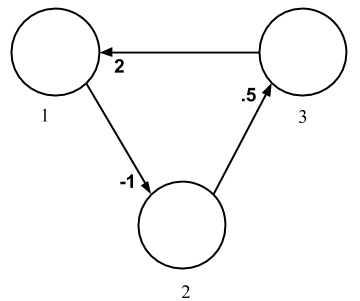
\includegraphics[scale=0.45]{./images/3NodeNet.png}
\caption[Jeff Yoshimi.]{A recurrent network with three nodes labelled $1,2,3$ and weights $w_{1,2} = -1, w_{2,3}=0.5, w_{3,1}=2$.}
\label{sampleNetRecurrent}
\end{figure}

\noindent
\stepcounter{LinearAlgebraCounter}
{\bf \theLinearAlgebraCounter.}  What is the matrix representation of the weights in the network in Fig. \ref{sampleNetRecurrent}?
{\bf Answer:}  
\[
\begin{pmatrix}
 0  &   -1 & 0 \\
 0  &   0 & 0.5 \\
 2  &   0 & 0 \\
\end{pmatrix}
\]
\bigskip

\noindent
\stepcounter{LinearAlgebraCounter}
{\bf \theLinearAlgebraCounter.}  What is the fan-in weight vector for node 2 in Fig. \ref{sampleNetRecurrent}?
{\bf Answer:}  $(-1)$. 
\bigskip

\noindent
\stepcounter{LinearAlgebraCounter}
{\bf \theLinearAlgebraCounter.}  What is
$\begin{pmatrix}1 & 1\end{pmatrix}\begin{pmatrix} 1 & 2  \\ 3 & 4 \end{pmatrix}$?
{\bf Answer:}  $\Big((1)(1) + (1)(3), (1)(2) + (1)(4)\Big)  = (4,6)$. 
\bigskip

\noindent
\stepcounter{LinearAlgebraCounter}
{\bf \theLinearAlgebraCounter.}  What is
$\begin{pmatrix}-1 & 1\end{pmatrix}\begin{pmatrix} 1 & -2  \\ 3 & 4 \end{pmatrix}$?
{\bf Answer:}  $\Big((-1)(1) + (1)(3), (-1)(-2) + (1)(4)\Big)  = (2,6)$. 
\bigskip

\noindent
\stepcounter{LinearAlgebraCounter}
{\bf \theLinearAlgebraCounter.}  What is
$\begin{pmatrix}-10 & 10\end{pmatrix}\begin{pmatrix} 0.5 & -0.5  \\ -1 &  1\end{pmatrix}$?
{\bf Answer:} $(-15,15)$. 
\bigskip


\noindent
\refstepcounter{LinearAlgebraCounter}\label{linAlgPractice1}
{\bf \theLinearAlgebraCounter.}  If the network in Fig. \ref{sampleNetRecurrent} has linear nodes and is given the activation vector $(a_1,a_2,a_3) = (1,1,1)$, what will its activation be in the next time step?
{\bf Answer:} 
\[
  \begin{matrix}\begin{pmatrix}1 & 1 & 1\end{pmatrix}\\\mbox{}\end{matrix}
 \begin{pmatrix}
 0  &   -1 & 0 \\
 0  &   0 & 0.5 \\
 2  &   0 & 0 \\
\end{pmatrix}
  =
  \bigg( (1)(0) + (1)(0) + (1)(2) ,\;\; (1)(-1) + (1)(0) + (1)(0) ,\;\; (1)(0) + (1)(.5) + (1)(0) \bigg)
  =  (2,-1,0.5)
\]
\bigskip

\noindent
\stepcounter{LinearAlgebraCounter}
{\bf \theLinearAlgebraCounter.}  If the network in Fig. \ref{sampleNetRecurrent} has linear nodes and is given the activation vector $(a_1,a_2,a_3) = (-1,-1,2)$, what will its activation be in the next time step?
{\bf Answer:} 
\[
  \begin{matrix}\begin{pmatrix}-1 & -1 & 2\end{pmatrix}\\\mbox{}\end{matrix}
 \begin{pmatrix}
 0  &   -1 & 0 \\
 0  &   0 & 0.5 \\
 2  &   0 & 0 \\
\end{pmatrix}
  =  (4,1,-0.5)
\]
\bigskip


\noindent
\refstepcounter{LinearAlgebraCounter}
{\bf \theLinearAlgebraCounter.}  If the network in question \ref{linAlgPractice1} is iterated four times, what will its activation be in those four time steps?
We saw from question \ref{linAlgPractice1} that after one time step the activation vector is $(2,-1,0.5)$. If we now use this as input to the network again we get:
\[
  \begin{matrix}
  \begin{pmatrix}2 & -1 & 0.5
  \end{pmatrix}\\\mbox{}
 \end{matrix}
 \begin{pmatrix}
 0  &   -1 & 0 \\
 0  &   0 & 0.5 \\
 2  &   0 & 0 \\
\end{pmatrix}
  =  (1,-2,-0.5)
\]
Repeating this process again with $(1,-2,-0.5)$ as input we get $(-1,-1,-1)$. Repeating one more time we get $(-2,1,-0.5)$.
{\bf Answer:}  $(2,-1,0.5),(-1,-2,-0.5),(-1,-1,-1),(-2,1,-0.5)$.
\bigskip
